\section{Object-oriented programming}

\label{sec:c++:oop}

The term \textit{object} generally means a (possibly empty) data type and
associated functions --- called \textit{methods} --- that operate on those data:
state and behavior\footnotemark.  The former can be as simple as the C
\texttt{struct}.  Methods are often (but may not be) available using the same
member access syntax.

\footnotetext{
    When coding, some programmers mix functional and imperative.  Others prefer
    not to: they believe in the separation of Church and state.  -{-} Robert
    Sewell}

\subsection{Method dispatch}

The first distinctive characteristic of object-oriented languages and systems is
that the behavior exhibited by an object is based on its ``type'', which may not
be known until the point where a method is called at runtime.

A common pattern in C is to augment \texttt{struct}s with members which are
function pointers taking as an argument the structure itself, by value or
pointer (listing \ref{lst:c++:method_ptrs}, figure \ref{fig:c++:method_ptrs}).
This pattern is very much similar to dynamic languages such as Lua, where each
object can have a distinct combination of method implementations.

While useful in some cases, this pattern is also needlessly wasteful when this
flexibility is not necessary and many instances of the \texttt{struct} (i.e.
objects) have the same values for their function pointer members.  The method
pointers are usually moved to a separate structure so that multiple objects can
refer to the unique combinations of method implementations (figure
\ref{fig:c++:vtable}).  This method-only structure is usually called a
\textit{virtual function table} (abbreviated as \textit{vtable}).

\begin{figure}[ht]
    \centering
    \begin{subfigure}[c]{0.5\textwidth}
        \begin{lstlisting}[
            style=c,
            label={lst:c++:method_ptrs},
            caption={Object with method pointers},
        ]
struct object {
    void (*method0)(struct object*);
    void (*method1)(struct object*);
    int data;
};

void f(struct object *o) {
    o->method0(o);
}
        \end{lstlisting}
    \end{subfigure}
    \begin{subfigure}[c]{0.35\textwidth}
        \begin{tikzpicture}[
            rectangle/.style={minimum height = 2em},
            >={Stealth[round]},
        ]
            \node[object = 3] (obj) at (0, 0) {
                \vrule height 0.5em depth 0.25em width 0pt
                \itshape obj
                \nodepart{two} \vrule height 0.5em depth 0.25em width 0pt
                method0
                \nodepart{three} \vrule height 0.5em depth 0.25em width 0pt
                method1
            };
            \node[rectangle,draw] (method0) at (3,  1) [rectangle] {method0};
            \node[rectangle,draw] (method1) at (3, -1) [rectangle] {method1};
            \draw[->] (obj.two east) -- (method0.west);
            \draw[->] (obj.three east) -- (method1.west);
        \end{tikzpicture}
    \end{subfigure}
    \caption{Object with method pointers}
    \label{fig:c++:method_ptrs}
\end{figure}

\begin{figure}[ht]
    \centering
    \begin{subfigure}[c]{0.45\textwidth}
        \begin{lstlisting}[
        style=c,
        label={lst:c++:vtable},
        caption={Object with virtual table pointer},
    ]
struct object {
    struct vtable *vptr;
    int data;
};

struct vtable {
    void (*method0)(struct object*);
    void (*method1)(struct object*);
};

void f(struct object *o) {
    o->vptr->method0(o);
}
        \end{lstlisting}
    \end{subfigure}
    \hspace{1em}
    \begin{subfigure}[c]{0.5\textwidth}
        \begin{tikzpicture}[
            rectangle/.style={minimum height = 2em},
            >={Stealth[round]},
        ]
            \node[object = 2] (obj) at (0, 0) {
                \vrule height 0.5em depth 0.25em width 0pt
                \itshape obj
                \nodepart{two} \vrule height 0.5em depth 0.25em width 0pt
                vptr
            };
            \node[object = 3] (vtable) at (3, 0) {
                \vrule height 0.5em depth 0.25em width 0pt
                \itshape vtable
                \nodepart{two} \vrule height 0.5em depth 0.25em width 0pt
                method0
                \nodepart{three} \vrule height 0.5em depth 0.25em width 0pt
                method1
            };
            \node[rectangle,draw] (method0) at (6,  1) [rectangle] {method0};
            \node[rectangle,draw] (method1) at (6, -1) [rectangle] {method1};
            \draw[->] (obj.two east) -- (vtable.one west);
            \draw[->] (vtable.two east) -- (method0.west);
            \draw[->] (vtable.three east) -- (method1.west);
        \end{tikzpicture}
    \end{subfigure}
    \caption{Object with virtual table pointer}
    \label{fig:c++:vtable}
\end{figure}

The benefit of this organization is the reduced storage requirement: each unique
list of function pointers is now stored once instead of being repeated in every
object.  This comes at the cost of an additional pointer dereference, which can
be alleviated by CPU caches for frequently-used tables.

Throughout this introductory section, excerpts from the Linux kernel will be
used as examples of a large C code base with several object-oriented
concepts\footnotemark.  \texttt{struct file} and \texttt{struct
file\_operations} (listing \ref{lst:c++:file}) are an example of the latter
pattern: the former contains it is responsible for implementing the various
types of files that a Unix/Linux system might have, while providing the generic
interface available through all file descriptors.

\footnotetext{V. \cite{Brown2011} for a thorough discussion.}

\begin{figure}[ht]
    \begin{lstlisting}[
        style=c,
        label={lst:c++:file},
        caption={\texttt{struct file\_operations}}
    ]
// include/linux/fs.h (with minor edits)
struct file {
    struct path f_path;
    struct inode *f_inode;
    const struct file_operations *f_op;
    // ...
};

// ...

struct file_operations {
    loff_t (*llseek)(struct file*, loff_t, int);
    ssize_t (*read)(struct file*, char*, size_t, loff_t*);
    ssize_t (*write)(struct file*, const char*, size_t, loff_t*);
    int (*mmap)(struct file*, struct vm_area_struct*);
    int (*open)(struct inode*, struct file*);
    int (*flush)(struct file*, fl_owner_t id);
    // ...
};
    \end{lstlisting}
\end{figure}

The structure should look familiar from the previous example.
\texttt{operations} is the usual suffix given to virtual table structures in
Linux.  One advantage of the manual implementation of object-oriented concepts
is the unlimited power to adapt the design, unimpeded by any assumptions or
constraints a more rigid language implementation might have.

\texttt{file\_operations} is a small example with respect to its members:
contrary to a virtual table in traditional object-oriented languages, many of
its method pointers can be \texttt{NULL}.  An unimplemented method in one of
those languages would (through different mechanisms depending on the particular
language) default to the implementation of its parent classes.  A low level
implementation is free to interpret a \texttt{NULL} value however suits it, and
this interpretation can vary per call site.  In the case of
\texttt{file\_operations}, the meaning of a \texttt{NULL} value varies for each
method:

\begin{itemize}
    \item \texttt{llseek}:
        A default operation is performed (modifying the position counter in
        \texttt{struct file}, in this case).  This is analogous to a default
        implementation in object-oriented languages, but note that the code is
        inlined in the caller and not executed by an indirect call.
    \item \texttt{read}:
        Signals that this object does not support the operation.
        \texttt{read(2)} calls will return \texttt{EINVAL}.
    \item \texttt{ioctl}/\texttt{unlocked\_ioctl}:
        An interface is being transitioned from one method to the other.  Both
        can coexist, although only one is ever set for any given object.  When
        all instantiations have been changed, the old method is removed.
    \item \texttt{aio\_read}/\texttt{aio\_write}:
        A similar case in that only one of the \texttt{read}/\texttt{write}
        methods or these are set: the asynchronous I/O API is such that one
        method can be implemented in terms of the other.  In this case, however,
        there is no transition and the two types of methods are expected to
        exist indefinitely.
    \item
        Finally, new operations added will default to \texttt{NULL} (v. section
        \secrefpar{subsec:c:literals}), so testing for that value can allow for
        incremental development.  A caller can immediately start using the new
        method when available while it can be progressively add to objects.
\end{itemize}

The defaulting of a method's implementation can also be effected in the
initialization of the virtual table object, instead of by treating the
\texttt{NULL} value specially.  A useful pattern in C is to provide a macro that
is placed at the beginning of a compound literal (listing
\ref{lst:c++:literal}).  This has the advantage that the calling code can avoid
a branch when calling the method, which will make the code shorter and faster
when skipping the indirect function call is not a common occurrence.

\begin{lstlisting}[
    style=c,
    label={lst:c++:literal},
    caption={Compound literal default macro},
]
#define DEFAULTS \
    .method0 = method0_default, \
    .method1 = method1_default

const struct vtable vtable = {DEFAULTS, .method0 = method0};
\end{lstlisting}

Another possibility when implementing virtual tables is to store more than
method pointers in them.  Some object-oriented languages do this internally to
support some level of reflection (e.g. \textit{run time type information}, RTTI,
in C++).  The type of information stored in this way is usually related to the
class of objects that share the virtual table.  \texttt{md\_personality} is one
such example in Linux (listing \ref{lst:c++:personality}): additional members
provide information such as a descriptive name and owning module, and intrusive
linked list pointers related to the registration of these virtual tables.

\begin{figure}[ht]
    \begin{lstlisting}[
        style=c,
        label={lst:c++:personality},
        caption={\texttt{struct md\_personality}}
    ]
// drivers/md/md.h (with minor edits)
struct md_personality {
    char *name;
    int level;
    struct list_head list;
    struct module *owner;
    bool (*make_request)(struct mddev *mddev, struct bio *bio);
    int (*run)(struct mddev *mddev);
    int (*start)(struct mddev *mddev);
    void (*free)(struct mddev *mddev, void *priv);
    void (*status)(struct seq_file *seq, struct mddev *mddev);
    // ...
};
    \end{lstlisting}
\end{figure}

\subsection{Inheritance}

Another aspect present in many object-oriented languages is the ability for
objects to inherit data and behavior from parent ``types''.  The relationship
between each level in the hierarchy with regards to how it operates on the
complete set of data and behavior can vary, from complete separation where every
level deals with only its own members, to more relaxed scenarios where different
levels cooperate to implement the full object functionality.

\subsubsection{\ident{union}}

The simplest implementation of data inheritance that is useful is the C
\texttt{union}: each possible combination of extra members is given its own
field in the union and users of the object decide somehow (via a discriminant
tag, based on context, etc.) which field to operate on (listing
\ref{lst:c++:data_inh_union}).  This implementation is simple and may be
preferred when a heterogeneous contiguous list of objects is required, but has
significant problems:

\begin{itemize}
    \item The structure has to be changed anytime a new implementation is added.
    \item
        Unions always occupy the size of its largest member, so every object
        will be as large as the largest ``child'' object.
\end{itemize}

\begin{figure}[ht]
    \begin{wrapfigure}{r}{0.5\textwidth}
        \centering
        \renewcommand{\arraystretch}{1.25}
        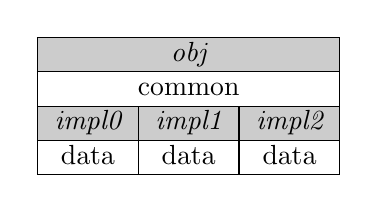
\begin{tikzpicture}[nodes={minimum height = 2em}]
            \node {
                \begin{tabular}{|c|c|c|}
                    \hline
                    \rowcolor{black!20}
                    \multicolumn{3}{|c|}{\itshape obj} \\ \hline
                    \multicolumn{3}{|c|}{common} \\ \hline
                    \rowcolor{black!20}
                    \itshape impl0 & \itshape impl1 & \itshape impl2 \\ \hline
                    data  & data  & data \\ \hline
                \end{tabular}
            };
        \end{tikzpicture}
        \renewcommand{\arraystretch}{1}
    \end{wrapfigure}
    \begin{lstlisting}[
        style=c,
        label={lst:c++:data_inh_union},
        caption={Data inheritance with \texttt{union}},
    ]
struct object {
    int common;
    union {
        struct object_impl0 impl0;
        struct object_impl1 impl1;
        struct object_impl2 impl2;
    } u;
};

struct object_impl0 { int data; };
struct object_impl1 { float data; };
struct object_impl2 { char *data; };
    \end{lstlisting}
\end{figure}

\subsubsection{\texttt{void*}}

One alternative solution fixes both problems, but introduces some of its own.  A
generic \texttt{void} pointer can be added to the structure, allowing client
code to set it to whatever value it wants.  This is seen in \texttt{struct
seq\_file} in the kernel, which is a utility for pseudo text files exposed in
the file system by the kernel, such as some files in \texttt{/proc}.
\texttt{seq\_open} (listing \ref{lst:c++:seq_open}) is used to initialize a
\texttt{seq\_file} based on the \texttt{struct file} we have seen before.
\texttt{file} has such a \texttt{void*} member called \texttt{private}, which is
used to store an object of the ``derived'' \texttt{struct seq\_file}.  It also
makes use of a virtual table called \texttt{struct seq\_operations}.

\texttt{seq\_file} in turn has its own \texttt{private\_data} member, which is
used by whatever code implements a particular path.  The utility function
\texttt{seq\_open\_private} further simplifies this process by
\texttt{kzalloc}ing a block of memory of the desired, calling \texttt{seq\_open}
setting its private pointer, and returning that pointer to the caller.
\texttt{kallsyms\_open}, for example, which implements \texttt{/proc/kallsyms},
attaches a \texttt{struct kallsyms\_iter} to the \texttt{seq\_file} it creates
(figure \ref{fig:cpp:kallsyms}).

While it solves the specific problem of the worst-case size for the structure,
there is now an extra pointer member, and the data attached to that pointer
potentially needs one to point back to the common structure as well.  It also
introduces the problem of where the extra data are stored, creating an
additional allocation in the worst case, and an additional memory dereference
when it has to be loaded.

\begin{figure}[p]
    \begin{lstlisting}[
        style=c,
        label={lst:c++:seq_open},
        caption=\texttt{seq\_open},
    ]
// fs/seq_file.c (with minor edits)
int seq_open(struct file *file, const struct seq_operations *op) {
    struct seq_file *p = file->private_data;
    if(!p) {
        p = kmalloc(sizeof(*p), GFP_KERNEL);
        if(!p)
            return -ENOMEM;
        file->private_data = p;
    }
    memset(p, 0, sizeof(*p));
    mutex_init(&p->lock);
    p->op = op;
    // ...
}
    \end{lstlisting}
\end{figure}

\begin{figure}[p]
    \centering
    \begin{tikzpicture}[
        rectangle/.style={minimum height = 2em},
        >={Stealth[round]},
    ]
        \node[object = 6] (file) at (0, 0) {
            \vrule height 0.5em depth 0.25em width 0pt
            \itshape file
            \nodepart{two} \vrule height 0.5em depth 0.25em width 0pt
            f\_path
            \nodepart{three} \vrule height 0.5em depth 0.25em width 0pt
            f\_op
            \nodepart{four} \vrule height 0.5em depth 0.25em width 0pt
            \ldots
            \nodepart{five} \vrule height 0.5em depth 0.25em width 0pt
            private\_data
            \nodepart{six} \vrule height 0.5em depth 0.25em width 0pt
            \ldots
        };
        \node[object = 6] (seq_file) at (4, 0) {
            \vrule height 0.5em depth 0.25em width 0pt
            \itshape seq\_file
            \nodepart{two} \vrule height 0.5em depth 0.25em width 0pt
            buf
            \nodepart{three} \vrule height 0.5em depth 0.25em width 0pt
            size
            \nodepart{four} \vrule height 0.5em depth 0.25em width 0pt
            \ldots
            \nodepart{five} \vrule height 0.5em depth 0.25em width 0pt
            private
            \nodepart{six} \vrule height 0.5em depth 0.25em width 0pt
            \ldots
        };
        \node[object = 3] (kallsyms_iter) at (8, 0) {
            \vrule height 0.5em depth 0.25em width 0pt
            \itshape kallsyms\_iter
            \nodepart{two} \vrule height 0.5em depth 0.25em width 0pt
            pos
            \nodepart{three} \vrule height 0.5em depth 0.25em width 0pt
            \ldots
        };
        \draw[->] (file.five east) -- (seq_file.one west);
        \draw[->] (seq_file.five east) -- (kallsyms_iter.one west);
    \end{tikzpicture}
    \caption{\texttt{kallsyms}}
    \label{fig:cpp:kallsyms}
\end{figure}

\begin{figure}[p]
    \begin{wrapfigure}{r}{0.6\textwidth}
        \centering
        \begin{tikzpicture}[every node/.style={
            object = 4,
            rectangle split part fill = {black!20, white, black!20, white},
        }]
            \node at (-2, 0) {
                \vrule height 0.5em depth 0.25em width 0pt
                \itshape obj0
                \nodepart{two} \vrule height 0.5em depth 0.25em width 0pt
                data
                \nodepart{three} \vrule height 0.5em depth 0.25em width 0pt
                \itshape object
                \nodepart{four} \vrule height 0.5em depth 0.25em width 0pt
                common
            };
            \node at (0, 0) {
                \vrule height 0.5em depth 0.25em width 0pt
                \itshape obj1
                \nodepart{two} \vrule height 0.5em depth 0.25em width 0pt
                data
                \nodepart{three} \vrule height 0.5em depth 0.25em width 0pt
                \itshape object
                \nodepart{four} \vrule height 0.5em depth 0.25em width 0pt
                common
            };
            \node at (2, 0) {
                \vrule height 0.5em depth 0.25em width 0pt
                \itshape obj2
                \nodepart{two} \vrule height 0.5em depth 0.25em width 0pt
                data
                \nodepart{three} \vrule height 0.5em depth 0.25em width 0pt
                \itshape object
                \nodepart{four} \vrule height 0.5em depth 0.25em width 0pt
                common
            };
        \end{tikzpicture}
    \end{wrapfigure}
    \begin{lstlisting}[
        style=c,
        label={lst:c++:data_inh_embed},
        caption={Data inheritance with embedded objects},
    ]
struct object { int common; };

struct object_impl0 {
    int data;
    struct object obj;
};

struct object_impl1 {
    float data;
    struct object obj;
};

struct object_impl2 {
    char *data;
    struct object obj;
};
    \end{lstlisting}
\end{figure}

\subsubsection{Base members}

Another solution to those problems is to invert the relationship between the two
structures: each ``derived'' object includes the base object somewhere in its
definition (listing \ref{lst:c++:data_inh_embed}).  Since the offset of the
member is a fixed-size constant known at compile time, the outer (base) object
can be found from a pointer to the inner with simple pointer arithmetic (listing
\ref{lst:c++:container_of}).  This turns an indirection at runtime to an offset
calculation at compile time.  The two objects are also adjacent in memory.

\begin{figure}[ht]
    \begin{lstlisting}[
        style=c,
        label={lst:c++:container_of},
        caption={\texttt{container\_of}},
    ]
#define container_of(p, type, member) \
    ((type*)((char*)(p) - offsetof(type, member)))

void f(struct object *o0) {
    struct object_impl0 *o = container_of(o0, struct object_impl0, obj);
    // ...
}
    \end{lstlisting}
\end{figure}

\begin{figure}[ht]
    \begin{wrapfigure}{r}{0.6\textwidth}
        \centering
        \begin{tikzpicture}
            \node[object = 3] at (-2.5, 0) {
                \vrule height 0.5em depth 0.25em width 0pt
                \itshape obj0/object
                \nodepart{two} \vrule height 0.75em depth 0.25em width 0pt
                common
                \nodepart{three} \vrule height 0.5em depth 0.25em width 0pt
                data
            };
            \node[object = 3] at (0, 0) {
                \vrule height 0.5em depth 0.25em width 0pt
                \itshape obj1/object
                \nodepart{two} \vrule height 0.75em depth 0.25em width 0pt
                common
                \nodepart{three} \vrule height 0.5em depth 0.25em width 0pt
                data
            };
            \node[object = 3] at (2.5, 0) {
                \vrule height 0.5em depth 0.25em width 0pt
                \itshape obj2/object
                \nodepart{two} \vrule height 0.75em depth 0.25em width 0pt
                common
                \nodepart{three} \vrule height 0.5em depth 0.25em width 0pt
                data
            };
        \end{tikzpicture}
    \end{wrapfigure}
    \begin{lstlisting}[
        style=c,
        label={lst:c++:data_inh_c++},
        caption={C++ data inheritance},
    ]
struct object { int common; };

struct object_impl0 {
    struct object obj;
    int data;
};

struct object_impl1 {
    struct object obj;
    float data;
};

struct object_impl2 {
    struct object obj;
    char *data;
};

void f(struct object*);

f(&(struct object_impl0){});
f(&(struct object_impl1){});
f(&(struct object_impl2){});
    \end{lstlisting}
\end{figure}

In particular, placing the base object at the beginning of the derived object
has several beneficial properties.  Both C and C++ guarantee that members
appearing in the same order at the beginning of two unrelated structures will
have the same offset and that a pointer to an object can be safely converted to
a pointer to the type of its first member\footnotemark.  This makes it ideal to
implement single inheritance as in C++ in this manner (listing
\ref{lst:c++:data_inh_c++}).  Since all base objects are prefixes of their
children, the base address of the derived is also a valid pointer to all of its
bases, and are guaranteed to be inter-convertible.

\footnotetext{
    C++ 20 introduced type traits specifically this verification:
    \texttt{std::is\_pointer\_interconvertible\_base\_of},
    \texttt{std::is\_pointer\_interconvertible\_with\_class}, and
    \texttt{std::is\_corresponding\_member}.}

One notable variation of this pattern, frequently found in C code, is to ensure
the common prefix using a macro which declares the fields, instead of using a
common structure.  This allows some flexibility in how these members and the
derived structures are embedded in other objects, at the cost of some
language/compiler support.  Listing \ref{lst:c++:tvaluefields} shows an example
from the implementation of object types in Lua.

\begin{figure}[ht]
    \centering
    \begin{subfigure}[t]{0.5\textwidth}
        \lstinputlisting[style=c, firstline=1, lastline=14]{cpp/lobject.h}
    \end{subfigure}
    \begin{subfigure}[t]{0.45\textwidth}
        \lstinputlisting[style=c, firstline=16]{cpp/lobject.h}
    \end{subfigure}
    \captionof{lstlisting}
        [\ident{TValuefields} in Lua]
        {\ident{TValuefields} in Lua (adapted from \ident{lobject.h})}
    \label{lst:c++:tvaluefields}
\end{figure}

\subsection{Multiple inheritance}

All types of inheritance shown so far involved a one-to-one relation between
base and derived objects.  Yet, sometimes it is desirable for an object to have
multiple bases, to combine methods and/or data from multiple other objects in
one, and it is not desirable to make either of those a base of the other(s).
With a large number of combinations, it may also be prohibitive to instantiate
all of the possible combinations a priori.

\begin{figure}[ht]
    \centering
    \begin{subfigure}[t]{0.4\textwidth}
        \begin{lstlisting}[style=c]
struct a { int data; };
struct b { int data; };
struct c { int data; };

struct d /* : a, b, c */ {
    struct a a;
    struct b b;
    struct c c;
    int data;
};

void f(d*);
        \end{lstlisting}
    \end{subfigure}
    \begin{subfigure}[t]{0.5\textwidth}
        \begin{lstlisting}[style=c]
int main(void) {
    struct d obj = {0};
    struct a *pa = &obj.a;
    // or pa = (struct *a)&obj
    struct b *pb = &obj.b;
    struct c *pc = &obj.c;
    struct d *pd = &obj;
    f((struct d*)pa);
    f(container_of(struct d, b, pb));
    f(container_of(struct d, c, pc));
    f(pd);
}
        \end{lstlisting}
    \end{subfigure}
    \captionof{lstlisting}{Multiple inheritance pointer adjustment}
    \label{lst:c++:multiple}
\end{figure}

While inheritance of data and behavior was kept largely separate in previous
sections, the implementation of multiple inheritance is more complex and often
combines both\footnotemark.  Consider the hierarchy in listing
\ref{lst:c++:multiple}.  A pointer to \texttt{d} and a pointer its \texttt{a}
portion are inter-convertible, since \texttt{a} is a common prefix of both.  A
pointer to \texttt{d} can obviously be used unchanged.  Obtaining a pointer to
\texttt{d} from a pointer to its \texttt{b} or \texttt{c} portion is not so
trivial.  The \texttt{container\_of} macro can be used here since the original
type of the object is known, but in general it could point to any object that
contains \texttt{b} or \texttt{c} objects at any offset, unknown at compile
time.  While the compile-time knowledge can be used for optimization (a process
called \textit{devirtualization}), this must often be a runtime calculation.

\footnotetext{
    The implementation in this section is based on \cite{Stroustrup1989}.}

The problem is fundamentally introduced by multiple inheritance: under regular
single inheritance, all objects in the hierarchy are inter-convertible, so the
same pointer can be passed to functions at any level.  In this example, however,
\texttt{d} could have a mixture of functions from \texttt{a}, \texttt{b}, and
\texttt{c}, and could override any of them (or one of its subclasses could).
Each method expects to receive a pointer to its corresponding type, and it is in
general impossible to determine the required offset for derived objects at
compile time.

Since these offsets are a property of the type and are used in function calls,
an obvious place to store them is the table of function pointers.  Each function
can have a different offset, so each entry will consist of the function pointer
and the object offset.  Calling a function no longer involves applying a fixed
offset --- the on in the virtual table must be used.  In addition, now the
object must have more than one table (one for each base) and the table for a
particular base type differs depending on the type of the derived object (as
they will have different offsets).  The root of the hierarchy can still share a
table with the derived object, so in this example a \texttt{d} object requires
three tables (one for \texttt{a}/\texttt{d}, one for \texttt{b}, and one for
\texttt{c}).

Listing \ref{lst:c++:multiple_call0} shows the base structures which can be used
to implement this:

\begin{figure}[ht]
    \lstinputlisting[
        style=c,
        firstline=3,
        lastline=18,
        label={lst:c++:multiple_call0},
        caption={Multiple inheritance function calls --- base structures},
    ]{cpp/mult_inh.c}
\end{figure}

\begin{description}
    \item[\texttt{vptr\_shared}]
        is a macro which declares both a base object and derived virtual table
        pointer as a \texttt{union} member.  This is valid since the base table
        is a prefix of the derived (it can be thought of as a "base object" of
        some sort), so pointers to them are inter-convertible.
    \item[\texttt{offset\_from\_base}]
        is a macro which calculates the offset from the address of a sub-object
        of a base type to the address of the object of the derived type.  This
        value will always be negative.
    \item[\texttt{call}]
        makes a virtual call through the virtual table of a sub-object of an
        object.
    \item[\texttt{vcall}]
        makes a virtual call through an object's primary virtual table.
    \item[\texttt{vfn}]
        is the implementation of an entry in the virtual table: a generic
        function pointer and an object pointer offset.
    \item[\texttt{voff}]
        applies a virtual table entry's offset to an object pointer.
\end{description}

\begin{figure}[ht]
    \lstinputlisting[
        style=c,
        firstline=19,
        lastline=28,
        label={lst:c++:multiple_call1},
        caption={Multiple inheritance function calls -- types},
    ]{cpp/mult_inh.c}
\end{figure}

With these definitions, the types and their corresponding virtual tables can be
declared (listing \ref{lst:c++:multiple_call1}).  The tables for \texttt{a},
\texttt{b}, and \texttt{c} are simple: they only contain virtual function
entries.  The table for \texttt{d} is slightly more complex: it is derived from
the \texttt{a} table, since those types can share the same table in \texttt{d}
objects.  Similarly, \texttt{a}, \texttt{b}, and \texttt{c} objects have normal
virtual table pointers, while \ident{vptr_shared} is used in \texttt{d} to
declare both the \texttt{a} sub-object and the pointer to the derived virtual
table.  The other sub-objects and members have simple declarations.

\begin{figure}[ht]
    \lstinputlisting[
        style=c,
        firstline=29,
        lastline=55,
        label={lst:c++:multiple_call2},
        caption={Multiple inheritance function calls --- virtual tables},
    ]{cpp/mult_inh.c}
\end{figure}

Listing \ref{lst:c++:multiple_call2} shows the definition of the virtual table
objects.  As expected from their declaration, the tables for \texttt{a},
\texttt{b}, and \texttt{c} contain only function pointers.  These entries have
no adjustment offset (all implicitly initialized to zero).

Because it uses multiple inheritance, \texttt{d} needs not a single virtual
table, but one for each of its bases.  The primary table contains its virtual
functions as well as an \texttt{a} virtual table.  None of the entries needs an
offset, since the \texttt{a} sub-object of \texttt{d} is at offset zero.  This
is different in the ``\texttt{b} in \texttt{d}'' and ``\texttt{c} in
\texttt{d}'' tables.  Because the sub-object offsets are not zero (they are
placed after the \texttt{a} part), entries for functions overridden in
\texttt{d} need an offset.  This is because those functions (in contrast to the
ones which are not overridden) expect a \texttt{d} object, while the fact that
the \texttt{b} or \texttt{c} table was used to arrive at this entry means the
calling code is dealing with a pointer to the corresponding sub-object.  Thus,
the table entry must contain a (negative) offset to the top of the \texttt{d}
object.

\begin{figure}[ht]
    \lstinputlisting[
        style=c,
        firstline=57,
        lastline=79,
        label={lst:c++:multiple_call3},
        caption={Multiple inheritance function calls},
    ]{cpp/mult_inh.c}
\end{figure}

Finally, listing \ref{lst:c++:multiple_call3} shows the calling code (or, more
realistically, what a compiler would generate from a higher level language).
Individual objects have their corresponding virtual table(s) appropriately
initialized, with the primary virtual pointer in \texttt{d} pointing to the
common \texttt{a}/\texttt{d} table.  These tables are then used for virtual
calls, either directly from the derived pointer or indirectly through a pointer
to a base sub-object, in which case the base has to be specified (this
information would be provided by the compiler in a language where virtual tables
are a primitive interface/implementation).

This solution works, but comes at a price.  \texttt{a}, \texttt{b}, and
\texttt{c} now have larger virtual tables since they could be used in a class
hierarchy, even though they don't themselves use multiple inheritance.  Both the
space and computation overhead is paid by all classes, regardless of their use.
To arrive at a better solution, it can be observed that only functions in
\texttt{d}'s table (the object which uses multiple inheritance) really need the
application of the offset: they are zero in all other tables.  The calculation
can be moved into a function prelude, which can in turn be used as the address
in the virtual table.  This restores the simple layout of tables for bases that
do not use multiple inheritance: they can simply contain the original function
pointers.

Listing \ref{lst:c++:multiple_opt} shows this optimization applied to the
previous example.  Virtual tables now contain only simple function pointers, and
overridden functions in the type which uses multiple inheritance now have
pointers to the prelude functions (which can be automatically generated by the
compiler).  \texttt{call} and \texttt{vcall} are also simpler since they can use
the input object pointer unmodified (note that the calling code does not
change from the previous example).

\begin{figure}[ht]
    \lstinputlisting[
        style=c,
        firstline=11,
        lastline=42,
        label={lst:c++:multiple_opt},
        caption={Multiple inheritance function calls (optimized)},
    ]{cpp/mult_opt.c}
\end{figure}
